
%%%%%%%%%%%%%%%%%%%%%%%%%%%%%%%%%%%%%%%%%%%%%%%%%%%%%%%%%%%
%%%%%%%%%%%%%%%%%%%%%%%%%%%%%%%%%%%%%%%%%%%%%%%%%%%%%%%%%%%
\subsection{XRD}
\begin{figure}
	\centering
	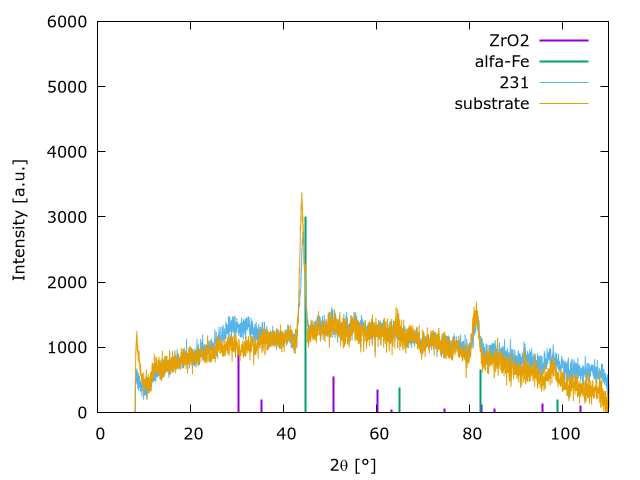
\includegraphics[width=\picwidth]{Pics/xrd.png}
	\caption{XRD spectra}
	\label{fig:xrd}
\end{figure}

%%%%%%%%%%%%%%%%%%%%%%%%%%%%%%%%%%%%%%%%%%%%%%%%%%%%%%%%%%%
%%%%%%%%%%%%%%%%%%%%%%%%%%%%%%%%%%%%%%%%%%%%%%%%%%%%%%%%%%%
\subsection{SEM}

%%%%%%%%%%%%%%%%%%%%%%%%%%%%%%%%%%%%%%%%%%%%%%%%%%%%%%%%%%%
%%%%%%%%%%%%%%%%%%%%%%%%%%%%%%%%%%%%%%%%%%%%%%%%%%%%%%%%%%%
\subsection{Material Scientific}
\subsubsection{First recipe} 
alteration of pH etc no improvement 

\subsubsection{Stability of the Solution}
\begin{itemize}
    \item compare AcOH vs AcOH+IPO 1:1 vs IPO (via boxplot) also G and phd? 
    \item p68 solution became clear after being milky 
    \item p74 
    \item why does IPO stabilize? 
    \item what is the reason for instability? 
    \item why does increased Zr conc decrease stability
    \item initial stirring time no influence on stability (and resulting layer?)
\end{itemize}

%%%%%%%%%%%%%%%%%%%%%%%%%%%%%%%%%%%%%%%%%%%%%%%%%%%%%%%%%%%
\subsubsection{Material}
\td{show results between 1ml acoh (199), acoh+ipo 1:1 (201) and ipo (192). Show graph of the three vs log pondus G and pinhole density and maybe distribution of single point measurements?}
\td{p68 iPrOH to milky solution and solution becomes clear!!!! checked how much 
is needed. 5F solution milky over night ~2ml, added 1ml IPO and clear.}
\td{instead of changing the stabilisation agent before optimisation, could change after pso, was vor und nachteile?}
\td{
so higher concentration of zro2 leads to less stable solution
5F ca 100min
4F ca 140min
3F ca 420min (7h)
}
- aquatic vs buthanolic: aquatic immidiately milky
\texttt{set boxwidth 2; set xtics 5; p "stat.dat" u 1:3 with boxes} 
\begin{itemize}
    \item double calcination (2x400C) was tried instead of pyrolization (4x200 then 400C),p49
\end{itemize}

%%%%%%%%%%%%%%%%%%%%%%%%%%%%%%%%%%%%%%%%%%%%%%%%%%%%%%%%%%%
%%%%%%%%%%%%%%%%%%%%%%%%%%%%%%%%%%%%%%%%%%%%%%%%%%%%%%%%%%%
\subsection{V-I and preoptimization}
\td{plot the predicted data for variables which should be excluded (Tcal, Vcal,Conc, layers)}
\td{varied doctor blading velocity: 10, 5, 1, 0.5, 0.2, 0.1. Slower less layer}
\todo{Following stirring times (in minutes) were tested and didn't have an influence on stability of the solution: 10-10-20, 10-10-45, 30-30-180.}
\td{extra PB-design with conc(2-4), layers(6-8), tcal(430-470), tvel(4-6),
vdoc(0.5-2), tdoc(40-60). low vdoc very homogenuous but actually nearly no 
deposition because miniscus is pulling liquid off the substrate.}
\td{IPO influence on "stability" p74: 600ul IPO makes clear, 4000 ul BuOH not clear with 
same base solution (1ml of 4F), added extra 400ul to BuOH sol and after 5min clear. 
of 1:5 is unacceptable Dilution }
- 21.8 (1F) from 15.02. 13:30 bis 
26.3 (1ml iPO to ca2ml of 5f) from 16.02. 16:30 bis 18.02.++
18.02 4F in 80min milky
      2F in ca 24h (stabilization AcOH)
- first recipe tried to improve to achieve more restisting layer. by pH value, surface 
tensionand solution ratios (only 10\% change because it was assumed, that the recipe is 
good and should be improved, but the recipe should be altered thoroughly.
two layers were also tried but didn't even pass the visual examination/test/inspection. 
A curst was produced. 
- At this point in time everything was doctor bladed by hand. The hight was varied (with tape).
When the switch to the erichsen was made. The height was kept constant in order to keep 
the variables to optimize ueberschuabar, but could have been even less variables.
If the movement was to slow the resluting  layer would be very inhomogenuous, thus the
velocity wasn't varied.
\td{p75 tested various vDOC (10,15,20) with TDOC (40,60,70,80) variations with only visual 
inspection of evaporation process. Ideally solution evaporate shortly after DB but not 
before} 
n-BuOH has boiling point of ca 117C\td{\cite{ncbi1butanol} look at source}
- p76, 146 (10x1F) good, 154 (3x4F) okay, 156 (3x3F) bad visualisation
- first experiments generated, but trashed because 1F solution neglected, contraints tightened
- p82 test to what extend AcOH can be replaced with iPOH
- 192 was first with IPOH
- why is IPO satbilizing? what are reasons for instability? 
\td{
acceptable layer was produced by buthanolic solution, but very unstable (short lived) how long? p41 
extra AcOH stabilzed but needed so much that dilution too large...
The stirring time was untersucht, but not much difference so shortest was used because 
short time can produces faster and the resulting solution is longer stable 
(after finishing mixing)
10 layers were tried of short stiring and gave good results? samples 130,131,134,135 (p43)
}
- \td{talk about the switch of recipe before emma: makes experiments hard/impossible to compare, but more practical and proof that it works weell} 


